\documentclass[11pt]{article}
\usepackage{amsmath}
\usepackage{amssymb}
\usepackage{amsthm}
\usepackage{amsfonts}
\usepackage[margin=1in]{geometry}
\usepackage{graphicx}
\usepackage[hidelinks]{hyperref}

\setlength{\parskip}{0.4em}

% Let a figure share a page with text instead of claiming one of its own.
\renewcommand{\topfraction}{0.92}
\renewcommand{\bottomfraction}{0.7}
\renewcommand{\textfraction}{0.07}
\renewcommand{\floatpagefraction}{0.85}

\title{Research Statement\\[0.3em]
\large Hierarchical and Adaptive Modelling for Protein--Drug Cofolding and Drug Design}
\author{Alireza Noroozi\\ \small anoroozi25@ku.edu.tr \quad https://alirzeanoroozi.github.io}
\date{October 2026}

\begin{document}

\maketitle

\section*{Motivation}

Predicting how a small molecule binds its protein target is one of the most important problems of
computational drug discovery. Cofolding models---AlphaFold3, Boltz, Chai---have
shown that a single network can jointly generate protein and ligand coordinates, and that doing so
outperforms the older pipeline of predicting a structure first and docking into it afterwards.
This is real progress, but it has arrived with a cost structure that now limits the field more than
the modelling ideas themselves do.

The cost is one of resolution. These models represent every atom of the system at every layer:
a 400-residue protein contributes on the order of three thousand heavy atoms, and attention over
that set dominates both training and inference. The consequence is that we train on far less data
than exists, with smaller models than we could otherwise afford, because the atomic representation
is applied uniformly---to the hydrophobic core, to flexible surface loops, and to the binding site
alike. Yet the information that determines binding is not uniformly distributed. A hydrogen bond
geometry three {\AA}ngstr\"om from the ligand decides whether a pose is right; the side-chain rotamer
of a solvent-exposed lysine forty {\AA}ngstr\"om away almost never does. We are paying full atomic
price for a whole structure in order to get a handful of contacts correct.

My research programme starts from this observation: \emph{resolution should follow information}.
I propose to build cofolding models that reason at multiple levels of abstraction within a single
system---coarse where the task is global geometry, atomic where the task is molecular recognition---and
that learn where to spend detail rather than having it specified by hand.

\begin{figure}[htbp]
\centering
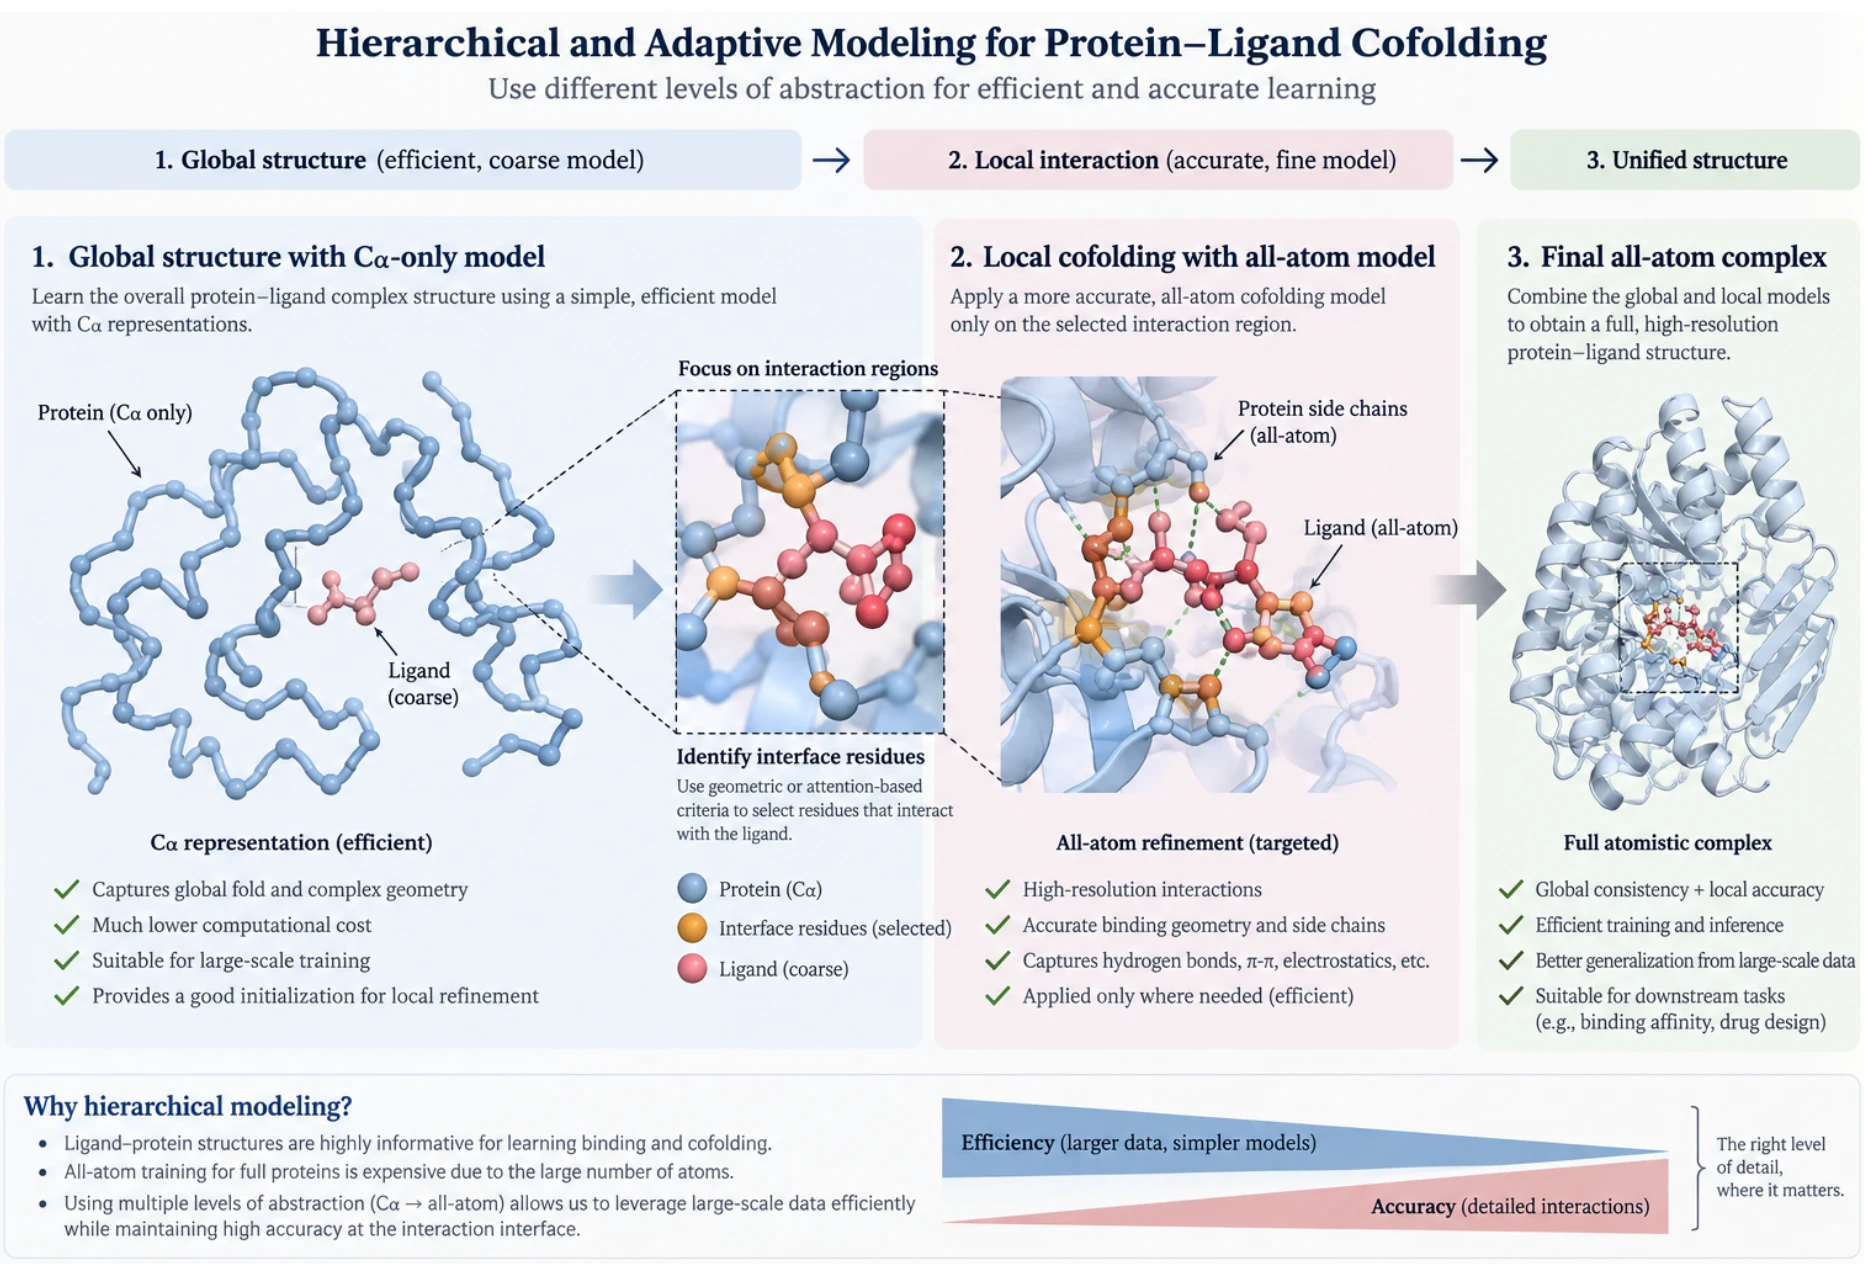
\includegraphics[width=0.9\textwidth]{hierarchical_cofolding.png}
\caption{Hierarchical cofolding. A coarse C$\alpha$-level model establishes the global complex
geometry and the approximate ligand placement; interface residues are then selected and refined with
an all-atom model; the two are recombined into a consistent full-resolution complex.}
\label{fig:overview}
\end{figure}

\section*{Proposed approach}

The programme decomposes into three stages, sketched in Figure~\ref{fig:overview}, each of which
raises its own research questions.

\subsection*{1. Global structure from a coarse model}

The first stage learns the overall fold of the complex and the approximate position of the ligand
using a reduced representation---C$\alpha$ traces for the protein, and a coarse-grained description
of the ligand such as pharmacophore-like beads or fragment centroids. Reducing the token count by
roughly an order of magnitude makes it feasible to train on substantially more data, to use larger
models under a fixed compute budget, and to run inference over large screening libraries.

The open question here is what \emph{must} be retained. A pure C$\alpha$ trace discards side-chain
identity, and with it much of what determines a pocket's shape and chemistry. I plan to study
intermediate representations---C$\alpha$ plus a learned per-residue embedding of side-chain
identity and approximate orientation, or a small fixed number of pseudo-atoms per residue---and to
characterise empirically how global placement accuracy degrades as representational detail is
removed. The aim is a principled answer to how coarse one can go before the coarse stage stops
being a useful initialisation for the fine one.

\subsection*{2. Adaptive selection of the interaction region}

The second stage decides where atomic detail is warranted. The simplest criterion is geometric:
select residues within a distance cutoff of the coarse ligand placement. This is a reasonable
baseline but a brittle one, since it inherits any error in the coarse stage and cannot recover a
pocket residue that the coarse model misplaced.

I am more interested in learned selection. The coarse model's own attention over the ligand tokens
is an obvious signal, and one that is available for free; a lightweight auxiliary head trained to
predict per-residue contact probability is another. Both admit a soft, probabilistic treatment in
which residues carry a continuous ``refine me'' weight rather than a binary label, and in which the
model can be calibrated to trade computational budget against the risk of excluding a residue that
mattered. The failure mode to characterise carefully is the asymmetric one: including an
unnecessary residue costs compute, while excluding a necessary one costs correctness. A selection
policy that is well calibrated on this asymmetry is, I think, the technically most interesting part
of the proposal.

\subsection*{3. All-atom refinement and consistent recombination}

The third stage applies a full all-atom cofolding model to the selected region only, resolving
side-chain conformations, hydrogen bonds, $\pi$--$\pi$ stacking, halogen bonds and electrostatic
complementarity at the resolution these interactions require. Because the region is small, this
model can be larger and run for more sampling steps per atom than a whole-complex model of the same
total cost.

Recombining the refined interface with the coarse global structure is not a matter of concatenation.
The refined region must remain geometrically consistent with the scaffold that surrounds it, and
the interface between the two resolutions is where artefacts will appear---bond-length and
chain-continuity violations at the boundary, or a refined pocket that no longer fits the coarse
fold. I plan to address this by making the boundary itself part of the learning problem: training
the fine model conditioned on the coarse context so that it is never free to drift, and applying a
short joint relaxation under a differentiable stereochemical objective. A useful test of whether
this works is self-consistency---re-running the coarse model on the refined complex should reproduce
the refined geometry.

\section*{Training, data and evaluation}

The hierarchy has a data consequence that I find as interesting as the efficiency one. Different
levels of abstraction can learn from different data. The coarse stage can be trained on the full
PDB, on predicted structures, and on the large body of complexes where the global fold is reliable
but atomic detail is not; the fine stage can be trained selectively on high-resolution crystal
structures where the interface geometry is actually trustworthy. This lets the model use the large
but noisy data where it is adequate, and the small but precise data where precision matters,
instead of forcing one training distribution to serve both.

For evaluation I intend to go beyond aggregate RMSD. The relevant questions for this architecture
are specific: at matched inference cost, does hierarchical cofolding achieve better pose accuracy
than a uniform all-atom model? Where does it fail---and are its failures concentrated in the coarse
stage's global placement or in the selection policy? I plan to report accuracy explicitly as a
function of compute, to stratify by pocket type and ligand flexibility, and to evaluate on
temporally held-out and low-homology targets rather than only on random splits, since the
generalisation claim is the one most easily overstated. Interaction-level metrics---whether specific
hydrogen bonds are recovered---matter more here than global superposition, because they are what
downstream affinity and design tasks depend on.

\section*{Longer-term direction}

Adaptive resolution is a general principle, and protein--ligand cofolding is where I want to
establish it rather than where I expect it to end. The same hierarchy applies to protein--protein
interfaces, to nucleic acid complexes, and to systems too large for uniform atomic treatment.
It also composes naturally with molecular dynamics, where coarse and fine representations have long
coexisted but have rarely been learned jointly, and it offers a route to conformational ensembles:
sampling cheaply at the coarse level and refining only the states that matter. Downstream, an
efficient and accurate cofolding model is the natural front end for binding affinity prediction and
for structure-based design, both of which are currently bottlenecked by the cost of generating
reliable complex structures at scale.

\section*{Background}

The three stages above map onto work I have already done, which is why I am confident the programme
is executable rather than merely appealing.

\textbf{Generative modelling over discrete biological sequences.} In \emph{AMP-DiT} (GenBio Workshop
at ICML 2026) I built a conditional discrete diffusion transformer that generates antimicrobial
peptides directly in sequence space, rather than inheriting representations from protein language
models trained on full-length proteins. Conditioning on a single activity classifier generalised
across several independent predictors, which indicated the model had learned antimicrobial structure
rather than the idiosyncrasies of one scorer. In \emph{IDPepDesign} I extended an insertion--deletion
diffusion model to target-conditioned peptide binder design with a pooled target representation and
residue-level cross-attention, improving perplexity from 17.1 to 11.3 and Fr\'echet protein distance
from 1.84 to 0.75 while producing competitive interface quality across eleven benchmark targets.
Both projects are exercises in exactly the question this proposal asks: what representation should a
generative model operate over, and what is lost when it is changed.

\textbf{Evaluation under conformational change.} During my research internship with the DELTA team at
Inria Nancy I worked on evaluating designed binders with molecular dynamics rather than
single-structure confidence scores, contributing to \emph{BinderEval} and to a new release of
\emph{COMPASS}. This is the part of the field that convinced me resolution and evaluation are the
same problem viewed from two sides: a static score cannot see induced fit, and a model that cannot
represent the interface at the right level of detail cannot be evaluated honestly at it either.

\textbf{Design against real targets, with experimental feedback.} In \emph{AMP-BindGen} I designed
peptide binders against the carbapenemases NDM-5 and KPC-3 in collaboration with clinical
microbiologists at Koç University, ranking candidates by a composite of interface confidence,
catalytic-site engagement, predicted activity and toxicity. Those designs went to the bench and
results have come back. I have also worked on protein--ligand systems directly, designing
protease-cleavable peptide linkers for antibody--drug conjugates in a covalently constrained
Fv--linker--payload assembly, which is a cofolding problem in all but name.

\textbf{Earlier foundations.} My BSc thesis on sequence-only paratope prediction with protein
language models was published in \emph{Scientific Reports}, and prior work on federated learning for
clinical data in \emph{IEEE JBHI} taught me to be careful about evaluation protocols when data are
scarce, heterogeneous and easy to overstate.

\section*{Fit}

I am drawn to this problem because it sits where machine learning architecture meets structural
biology: the central question---what level of detail does this part of the system actually
require?---is simultaneously a modelling question and a biophysical one, and I do not think it can be
answered well from either side alone. I would like to pursue it in a group working on structural or
generative modelling of biomolecules, and I am equally happy for the emphasis to fall on the
architectural and training side or on rigorous biophysical evaluation of what these models have and
have not learned. What I would bring is experience building generative models over biological
sequences from scratch, a habit of validating them against external predictors and wet-lab results
rather than only against the objective they were trained on, and a working familiarity with
molecular dynamics as a source of evidence rather than a post-hoc illustration.

\end{document}
